\section{curve-scalar}
\label{curve-scalar}

Take curve-secp256k1 as example, the same as other texs.

\begin{enumerate}
    \item target
        implement the multiplication between scalar and point. 
    \item constraints-logic
        \begin{figure}[!ht]
            \centering
            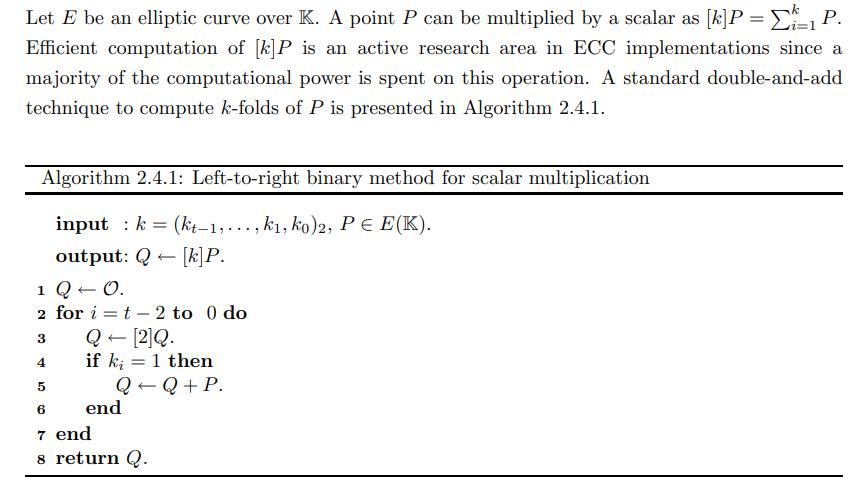
\includegraphics[width=0.8\textwidth]{curve-scalar.jpg}
            \caption{curve-scalar}
            \label{fig:curve-scalar}
        \end{figure}
    
    \item constraints-info and costs
        \begin{itemize}
            \item gate type num: 13 
            \item gate instance num: 180364          
        \end{itemize}
\end{enumerate}